\chapter{Miscellaneous}\label{chp:miscellaneous}

Variuous other small but useful algorithm, bascially from number theory and others.
\begin{compactenum}
    \item sieve of eratosthenes an other binary check ways
    \item gcd
    \item binary exponent for $O(log n)$ exponents
    \item Josephus puzzle
\end{compactenum}

\section{binary exponent}
excellent resource: 
    \href{https://cp-algorithms.com/algebra/binary-exp.html}{https://cp-algorithms.com/algebra/binary-exp.html}


\begin{marginfigure}
    \small
\begin{math}
    3^{13} = 3^{1101_2} = 3^8 \cdot 3^4 \cdot 3^1
\end{math}

\begin{align}
    3^1 &= 3 \\
    3^2 &= \left(3^1\right)^2 = 3^2 = 9 \\
    3^4 &= \left(3^2\right)^2 = 9^2 = 81 \\
    3^8 &= \left(3^4\right)^2 = 81^2 = 6561
\end{align}
\caption{Intution behind binary exponent}
\end{marginfigure}

\subsection{Recurrence Relation}
\begin{math}
    a^n = \begin{cases}
            1 &\text{if } n == 0 \\
            \left(a^{\frac{n}{2}}\right)^2 &\text{if } n > 0 \text{ and } n \text{ even}\\
            \left(a^{\frac{n - 1}{2}}\right)^2 \cdot a &\text{if } n > 0 \text{ and } n \text{ odd}\\
        \end{cases}
\end{math}

\subsection{Implementation,Recursion}
\begin{code2}
    long long binpow(long long a, long long n) {
        if (n == 0) return 1;

        long long res = binpow(a, n / 2);
        if (n % 2) return res * res * a; //ODD
        else return res * res; //EVEN
    }
\end{code2}


\subsection{Implementation,Iterative}
\begin{code2}
    long long binpow(long long a, long long n) {
        long long res = 1;
        while (n > 0) {
            if (n & 1) res = res * a;
            
            a = a * a;
            n >>= 1;
        }
        return res;
    }
\end{code2}

\section{Primality Test}
How do we check if a number if prime or not?

\begin{compactenum}
    \item simplest is to check,if the number if divisible by all number $<= 2 - num-1$
    \item If you observe, n/2 is the last number via which, you can divide n. Hence, we can check only upto n/2!
    \item 
\end{compactenum}

\subsection{Trail Division, Primality Test}
\begin{code2}
    bool isPrime(int x) {
        for (int d = 2; d * d <= x; d++) {
            if (x % d == 0)
                return false;
        }
        return x >= 2;
    }
\end{code2}

\subsection{Sieve of Eratosthenes}

Sieve of Eratosthenes is an algorithm for finding all the prime numbers in a segment $[1;n]$ using $O(n \log \log n)$ operations.

A number is prime, if none of the smaller prime numbers divides it. Since we iterate over the prime numbers in order, we already marked all numbers, which are divisible by at least one of the prime numbers, as divisible. Hence if we reach a cell and it is not marked, then it isn't divisible by any smaller prime number and therefore has to be prime.

\begin{marginfigure}
    
    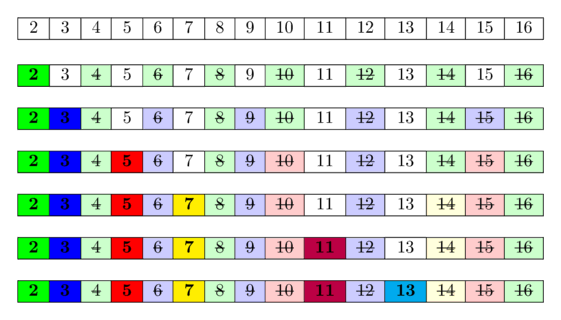
\includegraphics[width=\marginparwidth]{../resources/sieve_eratosthenes.png}
    \caption{A number is prime, if none of the smaller prime numbers divides it!}

\end{marginfigure}

\subsection{Implementation}
\begin{code2}
    int n;
    vector<bool> is_prime(n+1, true);
    is_prime[0] = is_prime[1] = false;
    for (int i = 2; i <= n; i++) {
        if (is_prime[i] && (long long)i * i <= n) {
            for (int j = i * i; j <= n; j += i)
                is_prime[j] = false;
        }
    }
\end{code2}

\section{GCD,LCM}

GCD stands for largest common divisor. i.e which is the largest number which can divide both number completely!

\begin{marginfigure}
    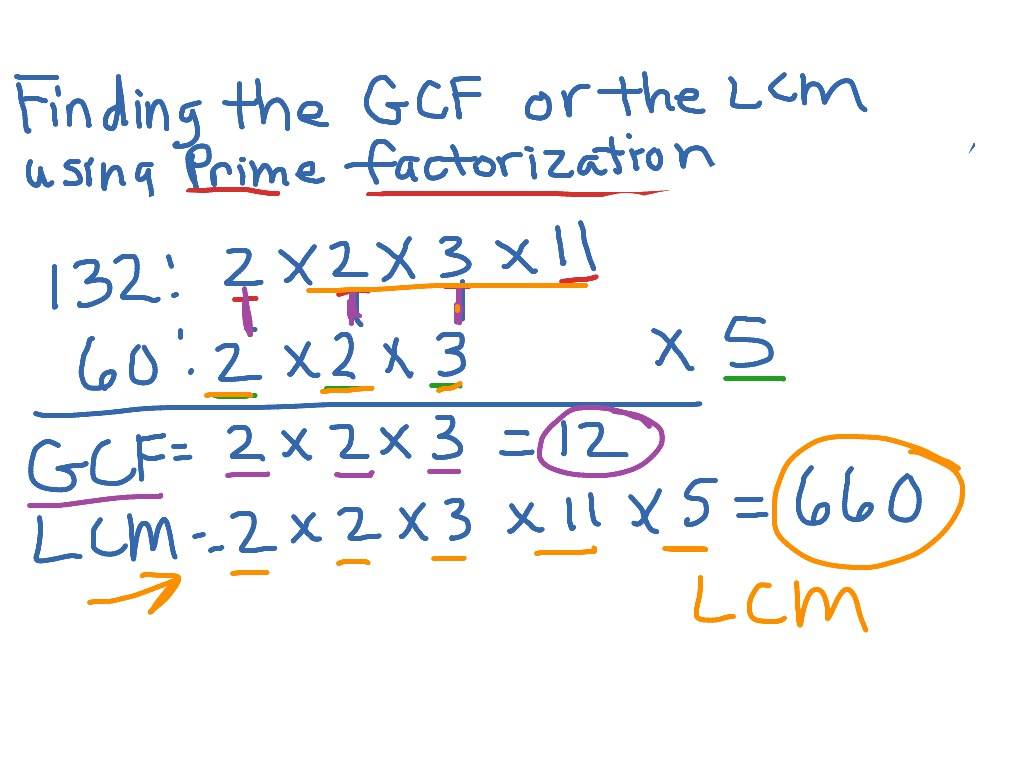
\includegraphics[width=\marginparwidth]{../resources/gcd_lcm.jpg}
    \caption{childhood prime factorization method to find gcd}
\end{marginfigure}

\subsection{Euclidean Algorithm}

Originally, the Euclidean algorithm was formulated as follows: subtract the smaller number from the larger one until one of the numbers is zero. Indeed, if $g$ divides $a$ and $b$, it also divide $a-b$.

On the other hand, if $g$ divides $a-b$ and $b$, then it also divides  $a = b + (a-b)$, which means that the sets of the common divisors of $\{a, b\}$ and $\{b,a-b\}$ coincide.

Note that $a$ remains the larger number until $b$ is subtracted from it at least $\left\lfloor\frac{a}{b}\right\rfloor$ times. Therefore, to speed things up, $a-b$ is substituted with $a-\left\lfloor\frac{a}{b}\right\rfloor b = a \bmod b$. 

Hence, the algorithm:
$$ \gcd(a, b) = \begin{cases}a,&\text{if }b = 0 \\ \gcd(b, a \bmod b),&\text{otherwise.}\end{cases} $$

\begin{code2}
    int gcd (int a, int b) {
        if (b == 0) return a;
        return gcd (b, a % b);
    }

    //c++ built-in gcd
    #include<numeric>
    gcd(a,b) OR lcm(a,b)
\end{code2}

\subsection{Extended Euclidean}
While the Euclidean algorithm calculates only the greatest common divisor (GCD) of two integers $a$ and $b$, the extended version also finds a way to represent GCD in terms of $a$ and $b$, i.e coefficients $x$ and $y$ for which: $$a \cdot x + b \cdot y = \gcd(a, b)$$

check out : \href{https://cp-algorithms.com/algebra/extended-euclid-algorithm.html}{https://cp-algorithms.com/algebra/extended-euclid-algorithm.html}

\subsection{Largest Common Divisor,lcm}
Having known how to find gcd, its wise to express lcm in gcd terms.

$$ \text{lcm}(a, b) = \frac{a \cdot b}{\gcd(a, b)} $$